\documentclass[a4paper,11pt]{article}
\pdfoutput=1 % if your are submitting a pdflatex (i.e. if you have
             % images in pdf, png or jpg format)

\usepackage{jcappub} % for details on the use of the package, please
                     % see the JCAP-author-manual

\usepackage[T1]{fontenc} % if needed



















\begin{document}
\maketitle
\flushbottom
\pagebreak
\section{Ricci scalar of previous rotating metric }
For our rotating metric (that was derived from visser and simpsons spherically symmetric metric ) you asked for the ricci scalar, I used an image, it looked the cleanest this way. You can use the zoom on overleaf to see it better
\begin{figure}[h]

    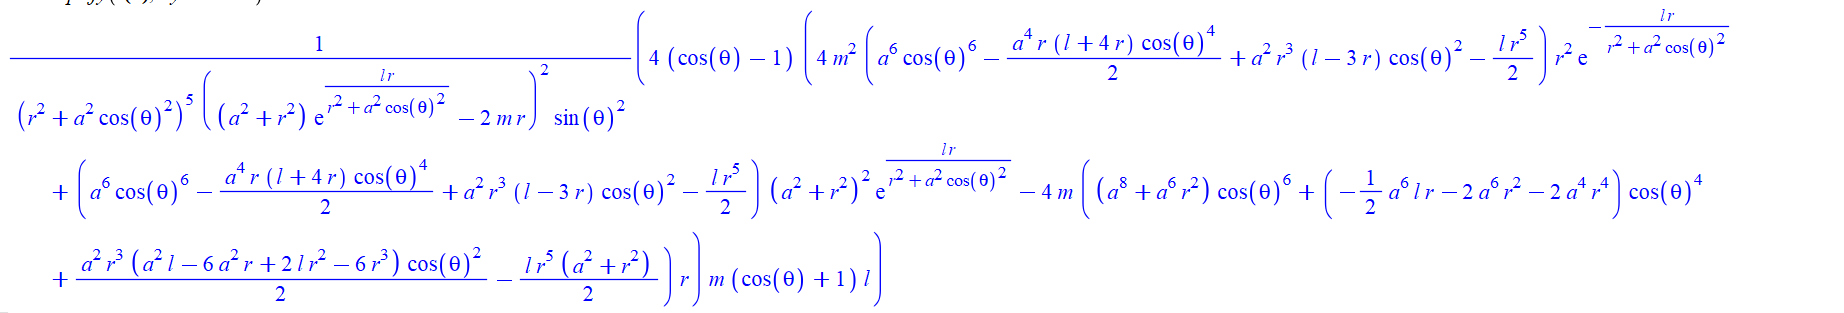
\includegraphics[scale =0.47]{MF&DF_Graphs/RS_NM.png}
    \caption{Ricci scalar of new rotating metric (the one based on simpson and vissers metric)}
    \label{fig:my_label}
\end{figure}
Here is the ricci scalar evaluated at $r=0$
\begin{equation}
\frac{4 \left(\cos\! \left(\theta \right)-1\right) m \left(\cos\! \left(\theta \right)+1\right) l}{a^{4} \cos\! \left(\theta \right)^{4} \sin\! \left(\theta \right)^{2}}  
\end{equation}
here is the ricci scalar evaluated at $\theta = \frac{\pi}{2}$
\begin{equation}
 -\frac{4 \left(-2 m^{2} l \,r^{7} {\mathrm e}^{-\frac{l}{r}}-\frac{l \,r^{5} \left(a^{2}+r^{2}\right)^{2} {\mathrm e}^{\frac{l}{r}}}{2}+2 m l \,r^{6} \left(a^{2}+r^{2}\right)\right) m l}{r^{10} \left(\left(a^{2}+r^{2}\right) {\mathrm e}^{\frac{l}{r}}-2 m r\right)^{2}}   
\end{equation}


\section{Ricci Scalar and Kretschmann scalar for any spherically symmetric metric with a mass function (and stress energy tensor) }
This is the Ricci scalar for any spherically symmetric metric of mass function $m(r)$ and it can be seen it goes to zero when $m(r)=constant$ which corresponds to the normal Schwarzschild solution. Which means any mass function that is not a constant will correspond to a none zero Ricci scalar and not be a vacuum solution.
\begin{equation}
  R =-  \frac{2 \left(r \left(\frac{d^{2}}{d r^{2}}m\! \left(r\right)\right)+2 \frac{d}{d r}m\! \left(r\right)\right)}{r^{2}}
\end{equation}
For the sake of completion this is the Kretschmann scalar for any spherically symmetric metric of mass function $m(r)$.
\begin{equation}
\frac{4 \left(\frac{d^{2}}{d r^{2}}m\! \left(r\right)\right)^{2} r^{4}-16 r^{2} \left(r \left(\frac{d}{d r}m\! \left(r\right)\right)-m\! \left(r\right)\right) \left(\frac{d^{2}}{d r^{2}}m\! \left(r\right)\right)+32 \left(\frac{d}{d r}m\! \left(r\right)\right)^{2} r^{2}-64 \left(\frac{d}{d r}m\! \left(r\right)\right) m\! \left(r\right) r+48 m\! \left(r\right)^{2}}{r^{6}}
\end{equation}
\\
\pagebreak
\\
The following is the stress energy tensor for a generic mass function in a spherically symmetric spacetime
\begin{equation}
T^{\mu}_{\nu}=
\begin{bmatrix}
P_{||} & 0 & 0 & 0 
\\
 0 & P_{\bot} & 0 & 0 
\\
 0 & 0 & P_{\bot} & 0 
\\
 0 & 0 & 0 & -\rho 
\end{bmatrix}
\end{equation}
\begin{equation}
T^{\mu}_{\nu}=
\begin{bmatrix}
-\frac{\frac{d}{d r}m\left(r\right)}{4 \mathrm{\pi} r^{2}} & 0 & 0 & 0 
\\
 0 & -\frac{\frac{d^{2}}{d r^{2}}m\left(r\right)}{8 \mathrm{\pi} r} & 0 & 0 
\\
 0 & 0 & -\frac{\frac{d^{2}}{d r^{2}}m\left(r\right)}{8 \mathrm{\pi} r} & 0 
\\
 0 & 0 & 0 & \frac{\frac{d}{d r}m\left(r\right)}{4 \mathrm{\pi} r^{2}} 
\end{bmatrix}
\end{equation}
\pagebreak
\section{General Minkowski core}
\subsection{new generalised Minkowski Core mass function and density}
An attempt to generate a new mass function that exhibits a Minkowski core. The Initial general starting function you suggested was the following. where $\alpha$ is dimensionless and $l$ is a Schwarzschild deviation parameter with dimensions length.
\begin{equation}
m_{\alpha}(r)=M (\tanh{(\alpha X)}+1)\frac{1}{2} \hspace{1cm}, X=\ln{(\frac{r}{l})}
\end{equation}
By substituting exponential and rearranging etc this becomes the following.
\begin{equation}
m_{\alpha}(r)=M ((\frac{e^{\alpha \ln{(r/l)}}-e^{-\alpha \ln{(r/l)}}}{e^{\alpha \ln{(r/l)}}+e^{-\alpha \ln{(r/l)}}})+1)\frac{1}{2}
\end{equation}
\begin{equation}
m_{\alpha}(r)=M (\frac{r^{2 \alpha}}{r^{2 \alpha}+l^{2 \alpha}})
\end{equation}
Where your initial suggestion corresponds to $\alpha = 1$. It can be seen that for any values of $\alpha$ this mass function satisfies the following
\begin{enumerate}
    \item $m_{\alpha}(0)=0$ Mass function is exactly 0 at exactly $r=0$
    \item $lim_{r \rightarrow \infty } (m_{\alpha}(r)) \rightarrow M$ Mass function always is  $M$ at asymptotic infinity 
    \item $lim_{r \rightarrow 0 } (\frac{2m_{\alpha}(r)}{r}) \rightarrow 0$ The ratio $m/r$ goes to 0 at $r=0$ which means the modified Schwarzschild metric is flat at $r=0$
    \item $l=0$ always recovers the standard Schwarzschild mass function $m(r)=M$
\end{enumerate}
\\
\\
Assuming a Spherically symmetric mass, we can define a generalised density by solving the following for $\rho$ using the derivative of the obtained mass function.
\begin{equation}
\rho_{\alpha}(r)=\frac{1}{4 \pi r^2}\frac{dm_{\alpha}}{dr}
\end{equation}
\begin{equation}
\rho_{\alpha}(r)=\frac{1}{4 \pi r^2}(\frac{2M \alpha l^{2 \alpha} r^{2 \alpha-1} }{(r^{2 \alpha}+l^{2 \alpha})^2})
\end{equation}
which leads to the following
\begin{equation}
\rho_{\alpha}(r)=\frac{M \alpha l^{2 \alpha} r^{2 \alpha-3} }{2 \pi (r^{2 \alpha}+l^{2 \alpha})^2}
\end{equation}
The value of $\alpha$ will have a strong impact on the behaviour of the energy density at/around $r=0$. The $r$ on the numerator determines this via its exponent. If the value of $\alpha$ makes the exponent negative then this will ensure the density is divergent at $r=0$. So we solve for $2 \alpha -3 > 0$ to find the values that correspond to a $0$ density core. 
\begin{enumerate}
    \item for $\alpha > \frac{3}{2}$ the density goes to 0 at the core, these are the values we are interested in.
    \item for $\alpha = \frac{3}{2}$ the density goes to a constant value at the core that value is $\rho_{\frac{3}{2}}(0) = \frac{\alpha}{2 \pi l^{2 \alpha}}$, so this could be a candidate de-Sitter core.
    \item for $\alpha < \frac{3}{2}$ the density diverges at $r=0$ due to the $r$ appearing on the denominator.
\end{enumerate}
\subsection{Generalised Event horizon and spherically symmetric metric}
The generalised line element is the following
\begin{equation}
    ds^2=-(1-\frac{2m_{\alpha}(r)}{r})dt^2+(1-\frac{2m_{\alpha}(r)}{r})^{-1}dr^2+r^2(d\theta^2+sin^2(\theta)d\phi^2)
\end{equation}
\begin{equation}
    ds^2=-(1-\frac{2M (\frac{r^{2 \alpha}}{r^{2 \alpha}+l^{2 \alpha}})}{r})dt^2+(1-\frac{2M (\frac{r^{2 \alpha}}{r^{2 \alpha}+l^{2 \alpha}})}{r})^{-1}dr^2+r^2(d\theta^2+sin^2(\theta)d\phi^2)
\end{equation}
 solving $g_{tt}=0$ gives you the general event horizon. Which is the solution to the following polynomial equation of order $2 \alpha$. For $l=0$ this reduces to $2M$
\begin{equation}
r^{2 \alpha}-2Mr^{2 \alpha - 1}+l^{2 \alpha}=0
\end{equation}
It can be seen that when $\alpha > 2 $ the polynomial will be degree higher than 4 which means it wont have an analytic solution.
\subsection{General Effective potential}
The general energy conservation equation takes the following form where $\epsilon = 0$ corresponds to light like particles and $\epsilon=1$ corresponds to time-like particles. $\mathcal{L}$ is the angular momentum per unit mass of the particle and $e$ is the energy per unit mass of the particle.
\begin{equation}
\Tilde{E}=\frac{1}{2}(e^2-\epsilon)=\frac{1}{2}(\frac{dr}{d\tau})^2-\epsilon \frac{m(r)}{r}+\frac{\mathcal{L}^2}{2r^2}-\frac{m(r)\mathcal{L}^2}{r^3}
\end{equation}
where the potentials take the following form. 
\begin{equation}
V(r)=-\frac{m(r)}{r}+\frac{\mathcal{L}^2}{2r^2}-\frac{m(r)\mathcal{L}^2}{r^3}
\end{equation}
\begin{equation}
V(r)=\frac{\mathcal{L}^2}{r^2}-\frac{2m(r)\mathcal{L}^2}{r^3}
\end{equation}
The first being for massive particles and the second being for light.
\section{The specific case of $\alpha = 2$}
I believe that $\alpha = 2$ is the best case to explore first. It greater than $3/2$, so will have a density of zero at the core and is the smallest integer that does so, leading to integer power equations for things like the horizon which is important in constraining $l$ analytically. 
\pagebreak
\subsection{Mass function, Density and metric}
The $\alpha = 2$ mass function takes the following form
\begin{equation}
 m(r)=M\frac{r^4}{r^4+l^4}
\end{equation}
When graphed this looks like the following
\\
\begin{figure}[h]
\centering
    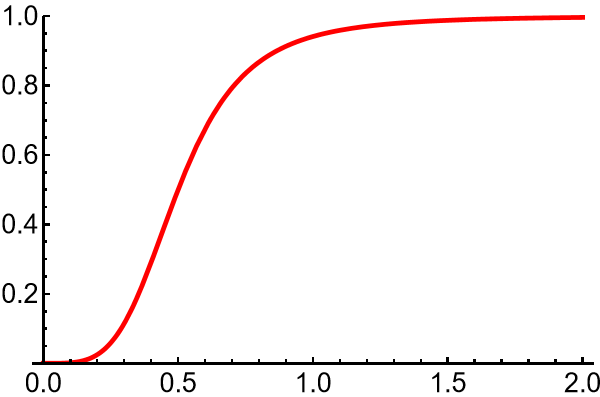
\includegraphics[width=8cm]{MF&DF_Graphs/Mass function.png}
    \caption{M(r) vs r}
    \label{fig:my_label}
\end{figure}
\\
\begin{equation}
\rho(r)=\frac{  Ml^{4} r }{ \pi (r^{4}+l^{4})^2}
\end{equation}
This has the property $\rho(0)=0$ and $lim_{r \rightarrow \infty}(\rho(r)) \rightarrow 0 $ as expected. When graphed this looks like the following
\begin{figure}[h]
\centering
    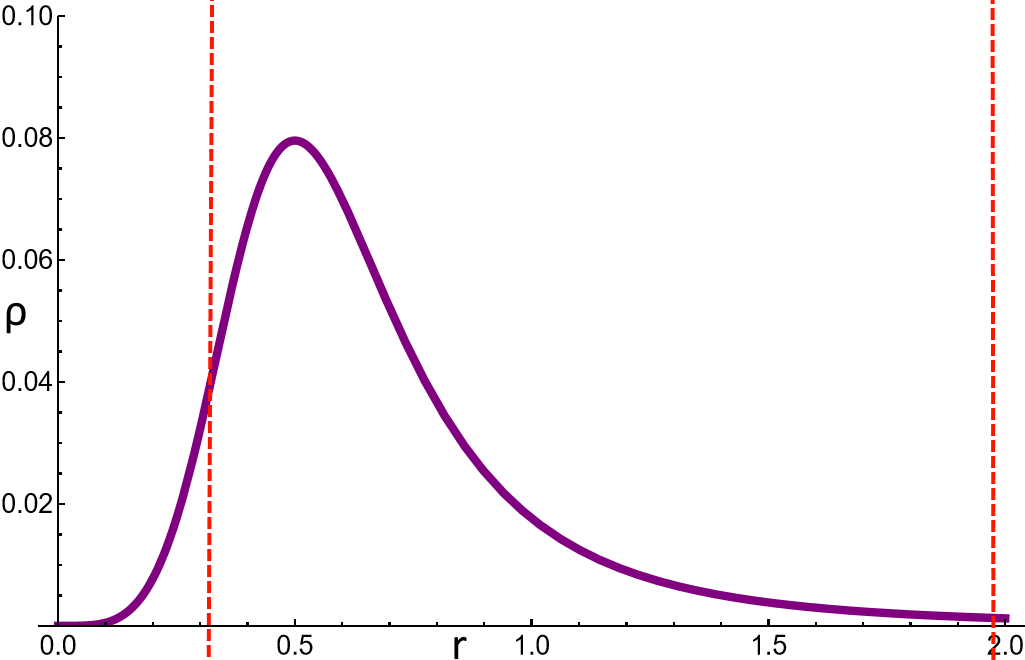
\includegraphics[width=10cm]{MF&DF_Graphs/DensityFunction.png}
    \caption{$\rho (r) vs r$ where $l=0.5 \& M=1$}
    \label{fig:my_label}
\end{figure}
\\
It has maxima at $r=\frac{l}{7^{\frac{1}{4}}}$ which is found by solving $\frac{d\rho}{dr}=0$ for r.
\\
The general line element for this metric with this mass function looks like the following
\begin{equation}
    ds^2=-(1-\frac{2M (\frac{r^{4}}{r^{4}+l^{4}})}{r})dt^2+(1-\frac{2M (\frac{r^{4}}{r^{4}+l^{4}})}{r})^{-1}dr^2+r^2(d\theta^2+sin^2(\theta)d\phi^2)
\end{equation}
This reduces to the Minkowski metric both at $r=0$ and $r\rightarrow \infty$. 

\subsection{Event horizons}
The Event horizon is given by the solution to the following.
\begin{equation}
    r^{4}-2Mr^{3}+l^{4}=0
\end{equation}
This is a quartic equation. It does have an analytic solution with 2 real roots for certain values of $l$ but this is incredibly large and unpractical. We can however find out for what values of $l$ the horizon dissolves. This is done using the quartic discriminant, When the discriminant is less than 0 ($D<0$), in the case of a quartic means there is 2 real roots (and two complex that we are not bothered with). The discriminant is the following
\begin{equation}
    D=256(1)^3(l^4)^3-27(-2M)^4(l^4)^3<0
\end{equation}
Which resolves to the following constraint on the ratio of $l/M$. This is the following
\begin{equation}
(\frac{l}{M})^4<\frac{27}{16}
\end{equation}
When this ratio is less than $\frac{27}{16}$, the geometry gives two event horizons, it becomes extremal at exactly that fraction and a horizonless object for greater than that value.

\subsection{Curvature Scalars}
Using Maple these curvature scalars are obtained. This is the ricci scalar for this geometry. 
\begin{equation}
R=\frac{8 l^{4} r M \left(5 l^{4}-3 r^{4}\right)}{\left(l^{4}+r^{4}\right)^{3}}
\end{equation}
the following is the Kretschmann scalar for the geometry. 
\begin{equation}
K=\frac{16 r^{2} M^{2} \left(19 l^{16}-56 l^{12} r^{4}+154 l^{8} r^{8}-24 l^{4} r^{12}+3 r^{16}\right)}{\left(l^{4}+r^{4}\right)^{6}}
\end{equation}

It can be seen from these both that the geometry is indeed singularity free at $r=0$

\subsection{Stress Energy tensor}
The Stress energy tensor looks like the following. 
\begin{equation}
T^{\mu}_{\nu}=
\begin{bmatrix}
P_{||} & 0 & 0 & 0 
\\
 0 & P_{\bot} & 0 & 0 
\\
 0 & 0 & P_{\bot} & 0 
\\
 0 & 0 & 0 & - \rho 
\end{bmatrix}
\end{equation}
\begin{equation}
T^{\mu}_{\nu}=
\begin{bmatrix}
-\frac{M \,l^{4} r}{\mathrm{\pi} \left(l^{4}+r^{4}\right)^{2}} & 0 & 0 & 0
\\
 0 & -\frac{\left(3 l^{4}-5 r^{4}\right) l^{4} r M}{2 \mathrm{\pi} \left(l^{4}+r^{4}\right)^{3}} & 0 & 0 
\\
 0 & 0 & -\frac{\left(3 l^{4}-5 r^{4}\right) l^{4} r M}{2 \mathrm{\pi} \left(l^{4}+r^{4}\right)^{3}} & 0 
\\
 0 & 0 & 0 & \frac{M \,l^{4} r}{\mathrm{\pi} \left(l^{4}+r^{4}\right)^{2}} 
 \end{bmatrix}{}
\end{equation}
 Both the energy density and the pressure are positive and related like $ \rho = -P_{||} $. similar to the other cases we have looked at.
\subsection{Energy conditions}
From Visser and Simpsons paper they discuss energy conditions, although not totally understanding much i compute them as they did. The energy density is always positive, so the weak energy condition is fulfilled
\subsubsection{Null energy condition}
In order to fulfil the null energy condition. Both $\rho + P_{||} \geq 0$ and $\rho + P_{\bot} \geq 0$ need to be satisfied globally. It can be seen immediately that $\rho + P_{||}$ will be positive globally. For the transverse pressure, we have the following when we calculate
\begin{equation}
r<(\frac{5}{3})^{\frac{1}{4}}l
\end{equation}
The transverse null energy condition is is violated in the deep core.
\subsubsection{Strong energy condition}
The strong energy condition requires that $\rho+P_{||}+2P_{\bot} \geq 0$ globally.  when you simplify and solve this you find that the strong energy condition is violated for $r<\frac{l}{(7)^{\frac{1}{4}}}$. Again the violation only occurs for the deep core. This is also the same value that the energy density has its maxima, maybe coincidence?  
\pagebreak
\subsection{Effective Potential}
The energy conservation equation looks like the following
\begin{equation}
\Tilde{E}=\frac{1}{2}(e^2-\epsilon)=\frac{1}{2}(\frac{dr}{d\tau})^2-\epsilon \frac{M(\frac{r^{2 \alpha}}{r^{2 \alpha}+l^{2 \alpha}})}{r}+\frac{\mathcal{L}^2}{2r^2}-\frac{M(\frac{r^{2 \alpha}}{r^{2 \alpha}+l^{2 \alpha}})\mathcal{L}^2}{r^3}
\end{equation}



\subsubsection{time-like}
\begin{equation}
V(r)=-\frac{M(\frac{r^{2 \alpha}}{r^{2 \alpha}+l^{2 \alpha}})}{r}+\frac{\mathcal{L}^2}{2r^2}-\frac{M(\frac{r^{2 \alpha}}{r^{2 \alpha}+l^{2 \alpha}})\mathcal{L}^2}{r^3}
\end{equation}

insert graph here
\subsubsection{light-like}
\begin{equation}
V(r)=\frac{\mathcal{L}^2}{r^2}-\frac{2M(\frac{r^{2 \alpha}}{r^{2 \alpha}+l^{2 \alpha}})\mathcal{L}^2}{r^3}
\end{equation}

Insert Graph here
\section{newman-janis of $\alpha = 2$}
In terms of a general spherically symmetric metric with a mass function, the only unique part about the newman janis algorthim is complexifying the mass function $m(r) \rightarrow m(r,\Bar{r})=m(r,\theta)$. I intend to explain and expand why i think this line element is the correct way to add rotation but initially i think this is what the line element should look like. where $a$ is the rotation parameter of the blackhole.
\centering
\begin{multline*}
{\displaystyle {\begin{aligned} ds^{2}=-\left(1-{\frac {2M(\frac{\Sigma^{2}}{\Sigma^{2}+l^4})r}{\Sigma }}\right)dt^{2}+{\frac {\Sigma }{\Delta }}dr^{2}+\Sigma d\theta ^{2}+\left(r^{2}+a^{2}+{\frac {2M(\frac{\Sigma^{2}}{\Sigma^{2}+l^4})ra^{2}}{\Sigma }}\sin ^{2}\theta \right)\sin ^{2}\theta \ d\phi ^{2} &\\ -{\frac {4M(\frac{\Sigma^{2}}{\Sigma^{2}+l^4})ra\sin ^{2}\theta }{\Sigma }}dt\,d\phi \end{aligned}}}	
\end{multline*}	
\begin{equation*}
\Sigma = r^2 +a^2\cos^2(\theta)
\end{equation*}

This form allows you to more easily see the transformed mass function $m(r,\theta)=M(\frac{\Sigma^{2}}{\Sigma^{2}+l^4})=M(\frac{(r^2 +a^2\cos^2(\theta))^{2}}{(r^2 +a^2\cos^2(\theta))^{2}+l^4})$ 
\\
\flushleft
This fulfils the basic requirements, such as reducing to Kerr when $l=0$ and the spherically symmetric version when $a=0$
\\
more simply the line element is 
\begin{multline*}
{\displaystyle {\begin{aligned} ds^{2}=-\left(1-{\frac {2M\Sigma r}{\Sigma^{2}+l^4 }}\right)dt^{2}+{\frac {\Sigma }{\Delta }}dr^{2}+\Sigma d\theta ^{2}+\left(r^{2}+a^{2}+{\frac {2M\Sigma ra^{2}}{\Sigma^{2}+l^4 }}\sin ^{2}\theta \right)\sin ^{2}\theta \ d\phi ^{2} &\\ -{\frac {4M\Sigma ra\sin ^{2}\theta }{\Sigma^{2}+l^4 }}dt\,d\phi \end{aligned}}}	
\end{multline*}	
More information regarding the horizons (Hopefully to constrain the ratio of $M,a$ and $l$ required for an event horizon to exist), curvature scalars and stress energy tensor will follow. Since this involves a lot of $\Sigma^2$ which involves an $r^4$, results will be of difficult or unsolvably high order. This is only for the $\alpha = 2$ choice from the spherically symmetric case. 
\\
\\
just like in the case of the metric by Simpson and Visser, you can produce a rotating metric like this or simply apply the old mass function to the Kerr metric like they did. So you can argue for another rotating candidate by simply taking the spherically symmetric $m(r)$ and using that in the Kerr metric, future comparison may decide if perhaps the other is better.
\\
\\
The effective potential should be easy to modify (being just a small modification of the kerr one) and i will try to do so at some point. 
\end{document}
